\section{Attribute, Zustand und Identität}
\label{sec:Kap-8.1}

Ein Software-Objekt 
\marginline{Software-Objekt}
hat eine eindeutige Identität, die es von anderen Objekten unterscheidbar macht. Es besitzt Attribute, in denen seine Daten gespeichert sind, kann wechselnde Zustände annehmen und verfügt über eine Menge von Operationen, die sein Verhalten bestimmen. 

\vspace{2mm} %% für Druck

Attribute und Operationen von Objekten werden in den Klassen 
\marginline{Klasse}
definiert. In Kapitel~4 haben wir das Konzept Klasse aus dem Blickwinkel der Realweltmodellierung betrachtet. Danach ist eine Klasse die Beschreibung der Abstraktion von Realwelt-Objekt zu modelliertem Objekt. Aus dem Blickwinkel des zu erstellenden Softwareprodukts ist eine Klasse wieder eine Beschreibung, und zwar die Beschreibung von Struktur und Verhalten von Software-Objekten. 

\vspace{2mm} %% für Druck

Eine Klasse definiert, welche Attribute, welche Operationen und welche möglichen Beziehungen zu anderen Objekten die ihr zugehörigen Objekte aufweisen sollen. Eine Klasse definiert außerdem einen Mechanismus – in der objektorientierten Programmierung als \textit{Konstruktor} bezeichnet – über den neue Objekte vom Typ der Klasse erzeugt werden können. Jedes zur Laufzeit der Software benötigte Objekt einer Klasse wird so anhand der Vorgaben der Klasse konstruiert. Diese Erzeugung neuer Objekte einer Klasse nennt man \textit{Instanziierung} und statt vom Objekt der Klasse spricht man in diesem Zusammenhang von der \textit{Instanz}
\marginline{Instanzen}
(manchmal auch vom \textit{Exemplar}) der Klasse. Der Begriff Instanz wird verwendet, wenn die Zugehörigkeit zu seiner Klasse betont werden soll („Eine Instanz der Klasse Katze“), weil damit zum Beispiel ausgedrückt werden soll, dass diese konkrete Instanz alle Eigenschaften besitzt, die die entsprechende Klasse definiert hat. Der Begriff Objekt wird in allgemeineren Zusammenhängen eingesetzt. 

\vspace{2mm} %% für Druck

Die \textit{Identität}
\marginline{Identität}
eines Objekts besteht ab dem Zeitpunkt seiner Erzeugung und ist unveränderlich in der Lebenszeit des Objekts. In vielen Programmiersprachen ist die Speicheradresse des Objekts das Kriterium seiner Identität. 

\sttpDefinitionskasten{\sttpDefinitionskastenSkalierungsfaktor}{Zustand eines Objekts}{Die Gesamtheit der aktuellen Wertebelegungen aller seiner \mbox{Attribute}}{Es gibt noch eine erweiterte Definition, die auch die Verbindungen des Objekts umfasst, also: „Die Gesamtheit der aktuellen Wertebelegungen aller seiner Attribute sowie seine bestehenden Verbindungen zu anderen Objekten.“ Die kurze Defini\-tion, die auch wir hier verwenden, entstammt einem implementierungsnahen Blickwinkel. Im Rahmen der Implementierung werden auch die Verbindungen zwischen Objekten auf Attribute abgebildet -- allerdings nicht zwingend auf Attribute dieses Objekts. Insofern sind es durchaus zwei unterschiedliche Defini\-tionen von Objektzustand.}

\clearpage %%% für Druck

Der \textit{Zustand} eines Objekts definiert sich über die Wertebelegungen seiner Attribute zum aktuellen Zeitpunkt. Daraus ergibt sich, dass sich der Zustand eines Objekts ändert, wenn sich mindestens der Wert eines seiner Attribute ändert. Unabhängig davon, wie häufig sich der Zustand eines Objekts in seiner Lebenszeit ändert, die Identität des Objekts ändert sich niemals. 

\vspace{2mm} %% für Druck

Wir 
\marginline{Identität vs. Zustand}
verdeutlichen die Konzepte Identität und Zustand an einem Beispiel. Abbildung~\ref{fig:identitaet_vs_zustand} schließt an das Autobeispiel aus Abschnitt~4.2 an und zeigt Auto-Objekte mit den beiden Attributen \sttpUMLText{modell} und \sttpUMLText{farbe}. Links sehen Sie das Objekt 
\linebreak %%% für Druck
\sttpUMLText{ellensAuto} mit dem Wert stahlblau im Attribut \sttpUMLText{farbe}. Ganz rechts sehen Sie ein anderes Objekt, nämlich das Objekt \sttpUMLText{heikesAuto} mit dem Wert rot im Attribut \sttpUMLText{farbe}. Es soll sich um zwei verschiedene Objekte handeln, jedes mit seiner eigenen Identität. In der Mitte der Abbildung betrachten wir erneut das Objekt \sttpUMLText{ellensAuto}, allerdings zu einem späteren Zeitpunkt als zum Zeitpunkt des linken Teils der Abbildung. Wir nehmen an, dass \sttpUMLText{ellensAuto} zu diesem zweiten Zeitpunkt umlackiert ist. Der Wert im Attribut \sttpUMLText{farbe} ist jetzt nicht mehr stahlblau, sondern rot. Durch die Änderung in diesem einem Attribut ändert sich der Zustand des Objekts \sttpUMLText{ellensAuto}, seine Identität aber nicht. Die Abbildungen links und in der Mitte beziehen sich also auf dasselbe Objekt.

\begin{figure}[h!]
	\centering
	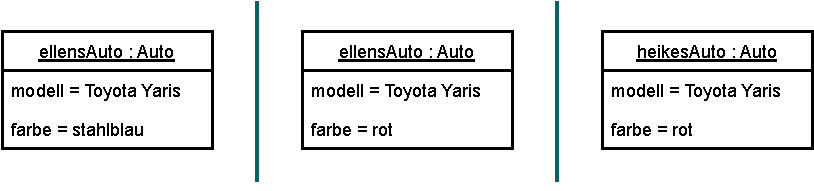
\includegraphics[scale=1.0]{Bilder/Kapitel-8/identitaet_vs_zustand.pdf}
	\vspace{\baselineskip} %% für Druck
	\caption[Zustand und Identität]{Ein Objekt zum Zeitpunkt t1 (links), dasselbe Objekt zum Zeitpunkt t2 in einem anderen Zustand (Mitte) und ein Objekt mit anderer Identität (rechts)}
	\label{fig:identitaet_vs_zustand}
\end{figure}

\sttpUMLText{ellensAuto} in der Mitte und \sttpUMLText{heikesAuto} rechts stimmen in den Wertebelegungen der beiden Attribute \sttpUMLText{modell} und \sttpUMLText{farbe} überein. Sie haben denselben Zustand, aber nicht dieselbe Identität. Die Änderung der Wertebelegung der Attribute eines Objekts hat keine Auswirkungen auf andere Objekte der Klasse. \sttpUMLText{heikesAuto} bleibt rot, auch wenn wir die Farbe von \sttpUMLText{ellensAuto} erneut ändern. Die beiden Objekte sind dann nur nicht mehr zustandsgleich.

\vspace{2mm} %% für Druck

Von der Zustandsgleichheit 
\marginline{Zustands\-gleichheit und referentielle Gleichheit}
zu unterscheiden, ist die sogenannte referentielle Gleichheit. Referentielle Gleichheit liegt vor, wenn sich hinter zwei unterschiedlichen 
\linebreak %%% für Druck
Objektnamen das identische Objekt verbirgt, es sich also nur um zwei Referenzen auf dasselbe Objekt handelt. Betrachten Sie Abbildung~\ref{fig:zustands_referentielle_gleichheit}.

\begin{figure}[h!]
	\centering
	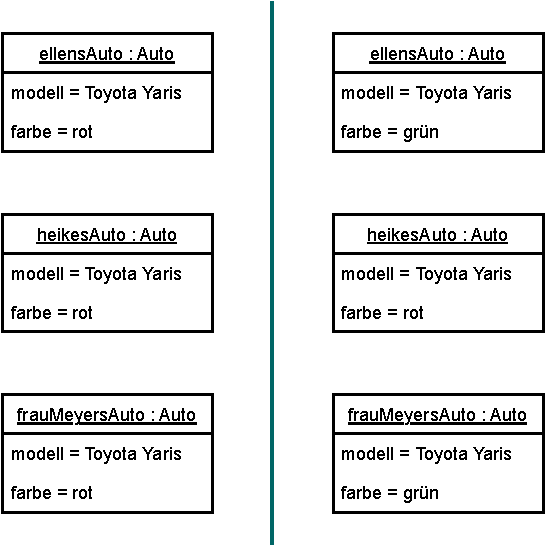
\includegraphics[scale=1.0]{Bilder/Kapitel-8/zustands_referentielle_gleichheit.pdf}
	\caption{Zustandsgleichheit und referentielle Gleichheit}
	\label{fig:zustands_referentielle_gleichheit}
\end{figure}

\pagebreak %%% für Druck

Links sind drei Auto-Objekte abgebildet: \sttpUMLText{ellensAuto}, \sttpUMLText{heikesAuto} und 
\linebreak %%% für Druck
\sttpUMLText{frauMeyersAuto}. Alle drei Objekte sind zustandsgleich. Wir ändern den Wert im Attribut \sttpUMLText{farbe} in \sttpUMLText{ellensAuto} von rot zu grün und erhalten die drei Objekte in den rechts abgebildeten Zuständen: \sttpUMLText{ellensAuto} ist grün, \sttpUMLText{heikesAuto} weiterhin rot, aber \sttpUMLText{frauMeyersAuto} plötzlich auch grün. Warum? Die Erklärung ist, dass es sich bei \sttpUMLText{ellensAuto} und \sttpUMLText{frauMeyersAuto} offensichtlich nicht um zwei unterschiedliche Objekte, sondern um dasselbe Objekt handelt, das in unserem Diagramm nur mit unterschiedlichen Namen gekennzeichnet wurde. Der Objektname ist nie gleichzusetzen mit der Identität des Objekts. Der Name ist lediglich ein Bezeichner, der das Objekt im Kontext (\zb im Diagramm, im Programmcode) identifiziert.

\vspace{2mm} %% für Druck

Manche 
\marginline{readOnly}
Eigenschaften von Realwelt-Objekten, wie zum Beispiel der Modelltyp \mbox{eines} Autos, ändern sich nicht. Bei der Abbildung einer Eigenschaft auf ein Software-Objekt möchte man eine solche Unveränderlichkeit vielleicht auch ausdrücken können. Die UML bietet dafür die textuelle Ergänzung \sttpUMLText{\{readOnly\}} an, die in der Klasse hinter dem Attribut notiert wird. Ein Beispiel dafür sehen Sie weiter hinten im Text in Abbildung~\ref{fig:klasse_auto_getter_setter}. Die Klasse Auto müsste dann natürlich später auch so implementiert werden, dass sichergestellt ist, dass jede Auto-Instanz einen Attributwert für \sttpUMLText{modell} enthält, dieser Wert aber während der Lebenszeit der Instanz nicht verändert werden kann. 